Para a implementação, inicialmente foram estudadas as possibilidades de serviços \emph{cloud}, como o Amazon, Linode e o Heroku. Dentre estes, o que se apresentou como o mais adequado para a implementação prática de um protótipo operacional de nosso mecanismo foi o Heroku. %\cite{heroku} é uma solução em \emph{cloud} que oferece a infra-estrutura como serviço de hospedagem, possibilitando desenvolvimento em \emph{frameworks} como \emph{django}, \emph{node.js} e \emph{Ruby on Rails}. Dentre estas alternativas, a implementação foi realizada em \emph{Ruby on Rails} (RoR), por maior experiência de membros do grupo e pela versatilidade da linguagem, que se mostra mais direta para a implementação, embora qualquer outro \emph{framework} e linguagem pudessem ser utilizados.
%
% A arquitetura do \emph{framework} RoR é completamente baseada no paradigma \emph{Model View Controler} (MVC), facilitando a organização dos módulos de nosso mecanismo. Desta forma, a estrutura do código escrito em RoR é composta de componentes de Modelo, de Visão e de Controle. Componentes de \textbf{modelo} correspondem aos dados - como eles são armazenados, obtidos, correlacionados. A parte de \textbf{visão} corresponde à parte gráfica da aplicação. Finalmente, \textbf{controladores} realizam a manipulação de dados como um todo, correspondem à parte lógica e funcional do código. Eles funcionam também como uma ponte entre modelo e visão, para que os dados transitem em ambos os sentidos.\\
%
Como \emph{framework}, foi utilizado o Ruby on Rails (RoR),  por ser baseado no paradigma baseado \emph{Model View Controler}, é fácil de criar a divisão necessária para os módulos do mecanismo. 

Desta maneira, o submódulo analizador de tráfego (AT) do mecanismo corresponde a um controlador. Uma requisição à aplicação será interceptada por esse componente de controle, que realizará a medição de algumas estatísticas e dados, e imediatamente em seguida, acionará o controlador que corresponde ao funcionamento da aplicação em si. Deve-se notar, contudo, que o tempo despendido neste controlador é ínfimo, é apenas o tempo necessário para processar algumas equações e salvar estes dados de controle. Em outras implementações, caso se perceba que o tempo afete o funcionamento do mecanismo de mitigação, este processamento pode ainda ser realizado em segundo plano.

Caso o AT detecte a existência de um possível ataque, uma nova instância \emph{cloud} é criada pelo submódulo INA e a aplicação replicada para esta, paralisando a aplicação original que passa a responder apenas como redirecionador. O processo de reinstanciação da aplicação pode ser obtido de duas maneiras. A abordagem mais simples seria a pré existência de uma segunda aplicação, sem nenhum recurso alocado. Entretanto, embora esta instância estaria pronta para que seus processos sejam escalados assim que necessário, esta abordagem não se comporta adequadamente no cenário de reinstanciação recursiva. A segunda abordagem envolve a hospedagem do projeto em um repositório do GitHub, que poderá ser clonado para a especificação da segunda instância a partir do código Ruby. 

Uma particularidade interessante do \emph{framework} RoR é a existência de um arquivo de configuração a cerca das rotas. A implementação do submódulo redirecionador de tráfego (RT) será realizada em cima deste arquivo, chamado \emph{routes.rb}. Para a exibição de qualquer página dinâmica da aplicação, o arquivo de rotas é inevitavelmente chamado. Desta forma, é o local ideal para a adição de clientes na \emph{blacklist} e respectiva filtragem dos clientes bloqueados pelo gerenciador da \emph{blacklist} (GB). No redirecionamento do tráfego para uma nova instância, uma entrada será adicionada, bloqueando o cliente em questão por determinado tempo.

% \begin{figure}[ht!]
% 	\centering
% 	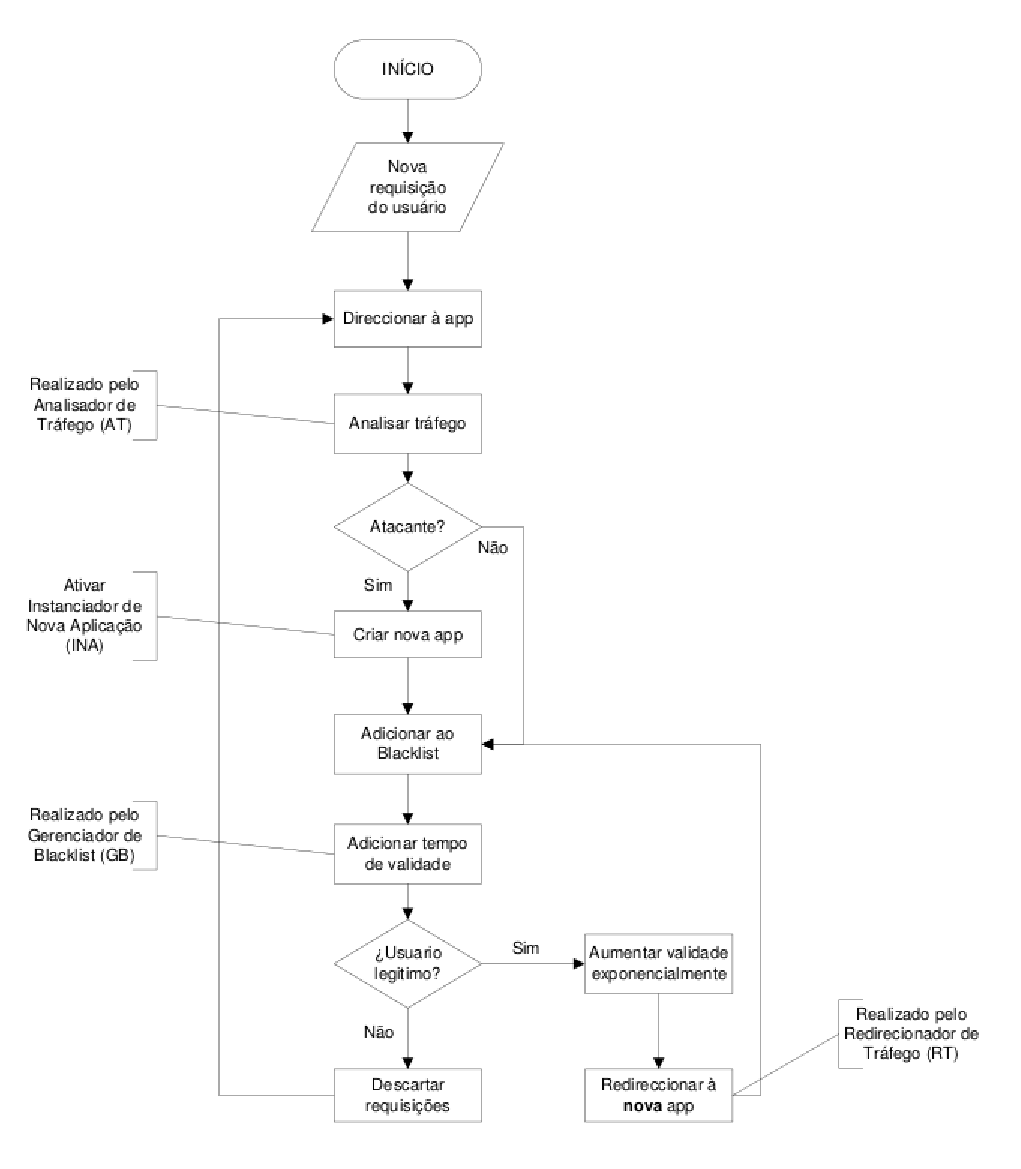
\includegraphics[width=0.55\textwidth]{images/dfd.eps}
% 	\hskip 1cm
% 	\caption{Funções da arquitetura de mitigação de DDoS}
% 	\label{fig:dfd}
% \end{figure}

A \emph{blacklist} em si e diversas outras variáveis de controle serão gerenciadas pela base de dados em \emph{cloud}~\cite{redis}. Esta base de dados é famosa pela sua simplicidade e eficiência. Ela basicamente mapeia \textbf{chave} e \textbf{dado}, oferecendo tempos de escrita e leitura correspondentes à \emph{hashing}. Desta forma, uma possibilidade para a implementação da \emph{blacklist} é o uso do Redis, utilizando o IP de um cliente como chave, e o tempo que este cliente permanecerá bloqueado como dado. Por ser, abstratamente, um mecanismo de \emph{hashing}, o tempo de checagem por um cliente será O(1), o que é excelente para um mecanismo que vai filtrar todo tráfego que chega à aplicação. %Uma visão estruturada das funções realizadas pela arquitetura proposta é descrita no diagrama de fluxo ilustrado na Figura~\ref{fig:dfd}.

Por fim, um aspecto interessante do uso do Heroku são os diversos \emph{addons} já customizados para o uso nele. Em particular, existe um \emph{addon} chamado \emph{New Relic} que é designado à coleta de diversas métricas para a análise de desempenho. Com seu uso, será possível saber com precisão o que se passa em todas as instâncias \emph{cloud} de uma perspectiva diretamente interna à esta \emph{cloud}. Assim, poderemos coletar dados não só da perspectiva externa à \emph{cloud}, perspectiva de usuário, como também, de perspectiva interna~à~ela.